\setcounter{section}{0}
\setcounter{dbltopnumber}{3}
\renewcommand{\thesection}{S\arabic{section}}
\setcounter{table}{0}\renewcommand{\thetable}{S\arabic{table}}
\setcounter{figure}{0}\renewcommand{\thefigure}{S\arabic{figure}}
\begin{center}
{\Large Supplementary material}\\[4pt]
{\normalsize Reference-Compatible Parallel Execution for Quantized LLM Inference}
\end{center}

\section{Deployments, Qualification and Sampling}
\subsection{References and execution profile}
The implementation fixes a numerical reference for each model/platform pair. Its identity includes the model and tokenizer bytes, prompt template, producer calls, device placement, numerical modules, KV type and capacity, output requests and stopping rules. CUDA references retain whole-prompt callers, physical microbatch one and last-only prompt output. Vulkan retains physical microbatch 128 and its original outer producer calls. The state profile is one dense, nonwrapping sequence with F16 K/V, greedy generation and non-flash attention.

W/L denotes whole-graph/local-attention cuts. L4/P denotes the Q8 backend-loop4/packed projection. M is target-only generation; D4 sets draft prefill microbatch four, independently of the proposal count $k$. The mixed-Q4 REF1-loop/group implementations retain one-column Q4\_K/Q6\_K arithmetic. Model hashes, exact runtime snapshots, compile commands and loaded-module identities are supplied by the companion records~\cite{records}.

\subsection{What numerical qualification observes}
The Linux Qwen/Smol deployment has 216 geometry vector comparisons and 6,524 natural-request vector comparisons, totaling 6,740 complete requested vectors. Its 4,784 state records cover active K/V by layer and logical position and the retained frontier. Four cut/projection M paths and both D4 paths pass these checks. The geometry panel spans widths 1, 4, 8 and 32, inside and crossing prefixes, tails and requested-output masks. Natural tests exercise first and later rejection, trim, pending corrections and bonus tokens, native EOG, caps and reset.

The Llama family transfer binds a separate reference and includes geometry, natural controls, independent EOG diagnostics, and heavy/clean execution comparisons. The mixed-Q4 target contains 385 Q4\_K, 65 Q6\_K and 257 F32 tensors; all six paths and 60 geometry cases qualify before timing. Its independent reference uses reserve one and candidates reserve 32, with C1024 and a common CUDA-Graphs-disabled policy. Transformer and output layers are GPU offloaded; the input embedding remains CPU mapped. Requested vectors contain 151,936 vocabulary entries, and active-state checks cover all 64 layers.

For speculative branches, an independently forced reference supplies the full target vector at each requested prefix. An autonomous reference supplies the emitted-token and stopping endpoint. Heavy numerical observations are collected outside clean performance runs; clean runs check endpoints, transaction traces, physical work, module identity and residency. The numerical evidence covers the declared fixtures and observation boundaries. It establishes the implementation's tested reference correspondence; the composition argument in the paper states the conditions needed at each subsequent phase.

\subsection{Input identities, warmup and order}
The Linux Qwen service and factorial panels reuse 16 pinned APPS/MATH task roots from the Windows study. The two scales therefore share input identities. The Llama service panel uses 12 roots selected after excluding prior project exposure. The live q8 panel uses a separate set of 16 roots, prompt length at most 192 and output cap 96. These selection statements concern project exposure. The 32B panel uses four exposed mathematics roots with cap 128; the structural append and equal-work panels use fixed development coordinates.

A Linux service worker loads its required target/draft resources once, performs two separate primer requests, then processes the test roots with the declared reset policy. The 32B panel instead places a full identical-root warmup immediately before each measured request. The four-arm factorial uses four Williams rows, balancing every position and all 12 directed within-row neighbors. The six-arm service studies use four rows with partial balance; the first Linux 8B study also retains fixed relative order between its two speculative arms. The balanced factorials supply component attribution.

Requests stop at native EOG or their token cap, retaining the observed output length. Resident-service, request-burst and worker clocks describe different inclusive windows. Synchronized phase diagnostics use disjoint host envelopes and a reconciled residual. Device-memory values are periodic global-device samples. Section~S6 lists the immutable sources and the statistics that can be reconstructed from the author package.

\section{Complete Application and Lifecycle Costs}
\begin{table*}[t]
\centering\footnotesize\tighttable
\caption{All six Linux application arms: mean measured resident seconds per request. Qwen panels have 64 requests per arm; Llama has 48. Each has four sessions. The first four columns are genuine target-only controls.}
\label{tab:allservice}
\begin{tabular}{@{}lrrrrrr@{}}\toprule
Model & W-L4-M & W-P-M & L-L4-M & L-P-M & W-L4-D4 & L-P-D4\\\midrule
\ApplicationRows
\bottomrule\end{tabular}
\end{table*}

The Qwen panels share the same 16 task identities for deployment and scale transfer. The Llama study selects 12 roots using its recorded project-exposure exclusions. The three application analyses use ratios of totals and 10,000 paired-root bootstrap draws. Each five-comparison family includes L-P-D4 against every fixed M and W-L4-D4. The fastest fixed M provides a descriptive summary; the five registered contrasts supply the inference.

The first Linux 8B study uses four cyclic six-arm rows; W-L4-D4 precedes L-P-D4 in each. Its two-D4 difference changes both factors and retains potential order effects. The balanced four-D4 studies supply factor attribution independently. Llama and 14B use four rows of a six-arm design with partial position/neighbor coverage; their direct application comparisons retain that conditional scope.

\begin{table*}[t]
\centering\footnotesize\tighttable
\caption{Complete-cost windows for representative fixed controls. Each entry is an aggregate within one study. Resident service, measured-request burst, worker and caller clocks overlap and must not be added. A dash means that this table does not include that field, not a measured zero.}
\label{tab:costs}
\begin{tabularx}{\textwidth}{@{}L{2.35cm}L{2.30cm}rrrY@{}}\toprule
Deployment & Fixed comparison & Resident service (s) & Request burst (s) & Native workers (s) & Window interpretation\\\midrule
Linux Qwen3-8B & W-P-M / L-P-D4 & 172.146 / 142.523 & --- & 200.739 / 168.973 & Worker totals shown at reported millisecond precision.\\
Linux Qwen3-14B & W-P-M / L-P-D4 & 294.542 / 219.318 & 294.632 / 219.405 & 662.546 / 594.559 & Same registered requests; worker includes integrity, loading and primers.\\
Linux Llama-8B & L-P-M / L-P-D4 & 136.873 / 121.102 & --- & 361.717 / 368.822 & Resident improvement does not preserve the process-level ranking.\\
Windows Qwen3-8B & W-P-M / L-P-D4 & 219.810 / 155.814 & 220.178 / 156.126 & 260.240 / 192.568 & Windows measurements; task records reused for Linux, with separate references.\\\bottomrule
\end{tabularx}
\end{table*}

The Windows practical panel originally selected 16 new roots, four sessions, four real target-only M controls, one matched-residency M and L-P-D4. Its mean fixed-M times are 3.483689, 3.434533, 3.511301 and 3.474824\,s; L-P-D4 averages 2.434597\,s. The four-comparison adjusted root intervals support the reported resident-service direction. The added draft requires more initialization and sampled memory; its per-worker setup difference is approximately 0.420\,s and device-global sampled peak difference approximately 0.705\,GiB. The memory difference is a device-global sampled value; per-process peaks and energy were not measured.

The complete Windows 64-request phase account gives target savings 96.889\,s, draft additions 31.931\,s and other net additions 0.962\,s, yielding 63.996\,s of resident savings. In the two-root synchronized Vulkan cost diagnostic, target savings 0.466681\,s are offset by draft additions 1.923330\,s and other additions 0.210582\,s. The synchronized diagnostic and the four-root clean Vulkan pilot use distinct measurement windows and are reported separately.

\section{Factorial and Mixed-Q4 Results}
\begin{table}[t]
\centering\footnotesize\tighttable
\caption{All fixed effects from the balanced Qwen D4 panels. Ratios below 1 favor the numerator; intervals are 99\% family-adjusted paired-root percentiles. P denotes packing.}
\begin{tabular}{@{}llrl@{}}\toprule
Model & Fixed-factor comparison & Ratio & Interval\\\midrule
\FactorRows
\bottomrule\end{tabular}
\end{table}

Each factorial uses the same 16 task roots, four arms and four Williams rows, with two separate primers per worker: 256 formal requests plus 32 primers. The per-session arm orders balance all four positions and all 12 directed within-session neighbors. The interaction estimand is the equal-root geometric mean of $(L_P/W_P)/(L_{L4}/W_{L4})$. Its 8B estimate is 1.000696 with interval [1.000069, 1.001393]; the 14B estimate is 1.001703 with interval [1.000293, 1.003338]. Both interactions indicate mild attenuation of the combined effect. Figure~\ref{fig:factorial} includes every root-level ratio.

\begin{table*}[t]
\centering\footnotesize\tighttable
\caption{Complete 32B mixed-Q4 costs. Each arm has 16 measured requests and 16 full identical-root immediate warmups. Worker and caller totals include the warmups and initialization. They are not additional independent task observations.}
\label{tab:q32all}
\begin{tabular}{@{}lrrrr@{}}\toprule
Arm & Measured service sum (s) & Mean service (s) & Native-worker sum (s) & Caller sum (s)\\\midrule
\QThreeTwoRows
\bottomrule\end{tabular}
\end{table*}

\begin{figure}[t]
\centering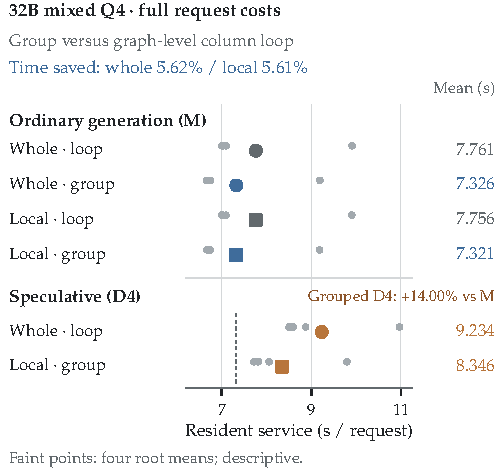
\includegraphics[width=\columnwidth]{figures/mixed_q4.pdf}
\caption{All six mixed-Q4 service paths. Markers and values give mean resident time; faint points are four root means over four rounds. The loop comparison executes scalar columns through separate graphs. Grouped ordinary generation is fastest, while grouped D4 takes 14.00\% more service than the fastest M.}
\label{fig:s-mixed}
\end{figure}

The 32B reference is pristine Linux scalar execution with UB1/reserve 1. The candidates use UB32/reserve 32, C1024, F16 KV, no flash and a common graphs-disabled policy fixed before timing. The graph-level REF1-loop and independent REF1-group retain the per-type scalar dot functions and the original activation quantizer. The 5.61\% comparison uses graph-level scalar-column execution. The precise candidate source modification is in graph lowering; unchanged CUDA archive members are bound in the build record. Each requested full output and active state in the finite qualification is checked against this deployment's own reference.

The four exposed roots are short mathematics inputs. Whole/group and local/group improve ordinary service by 5.616\% and 5.606\% relative to their respective graph-level loops. At fixed projection, L/W differs by approximately 0.055\%--0.067\%. L-REF1-group-D4 takes 9.614\% less service than W-REF1-loop-D4, a compound comparison, but 14.000\% more than the strongest M. Table~\ref{tab:q32all} includes all six paths. Model size, quantization, recipe and graph policy jointly distinguish this deployment from the 14B Q8 study.


\subsection{Backend-internal loop: completed operator follow-up}
The follow-up at \texttt{f419a89d} fixes whole lowering and scalar-column arithmetic. G loops in the graph; B quantizes once and dispatches scalar dots inside the backend; C groups independent columns. After S1 qualification (243 workers, 783 operations), S2 completes three matched blocks in four exposed tensor cells: 36 fresh workers, each with one warmup and one measurement, all with CUDA Graphs off.

\begin{table}[t]
\centering\footnotesize\tighttable
\caption{Strong-loop operator comparison. B/G and C/B are geometric means of three paired elapsed-time ratios. The final column gives the observed C/B minimum--maximum, not a confidence interval. All four exposed cells are shown.}
\label{tab:strong-operator}
\begin{tabular}{@{}llrrl@{}}\toprule
Type & Width & B/G & C/B & C/B range\\\midrule
\StrongSTwoRows
\bottomrule\end{tabular}
\end{table}

B/G and C/B have equal-cell geometric ratios of 0.6390 and 0.8528 (Table~\ref{tab:strong-operator}); Q6\_K/$q=4$ has mixed paired directions. These one-warmup operator results complement the 5.61\% graph-loop service comparison. At the evidence cutoff, the full-model backend-loop comparison remains in progress. The completed matched-history A5000 width panel is reported in Section~S4. The package recomputes the operator summaries from the published block ratios.

\section{Verification Width}
\begin{table}[t]
\centering\footnotesize\tighttable
\caption{All eight Windows width-study arms. Each arm has 128 formal requests: 16 roots across eight order blocks. The candidate output reservation is 8 for both k3 and k7.}
\begin{tabular}{@{}lrr@{}}\toprule
Arm & Service sum (s) & Mean (s)\\\midrule
\QEightRows
\bottomrule\end{tabular}
\end{table}

\begin{table}[t]
\centering\footnotesize\tighttable
\caption{Registered fixed-k7 secondary comparisons. Their 98.75\% adjusted intervals belong to a separate four-comparison family and all contain 1.}
\begin{tabular}{@{}lrl@{}}\toprule
Comparison & Ratio & Interval\\\midrule
\QEightSecondaryRows
\bottomrule\end{tabular}
\end{table}

\begin{figure}[t]
\centering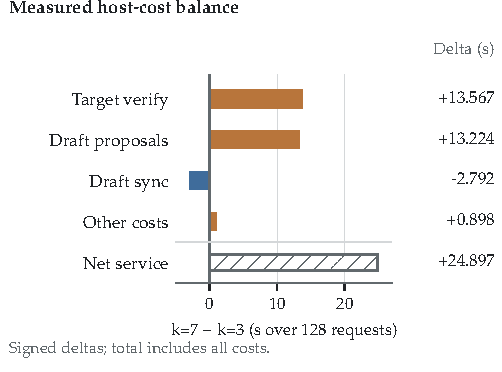
\includegraphics[width=\columnwidth]{figures/supp_width_cost.pdf}
\caption{LOCAL-packed host-cost difference over 128 requests. Bars and values give k7 minus k3; negative values save time. Other costs include prefill, output ownership, setup/teardown and the remaining residual. These measured phases include host work, synchronization and GPU execution.}
\label{fig:s-widthcost}
\end{figure}

Each arm emits 11,472 tokens. The corresponding k3/k7 counts are 3,504/2,296 verification cycles, 10,512/16,072 proposed tokens, 7,928/9,152 accepted proposals, 1,136/1,256 first inspected mismatches and 1,448/5,664 unconsumed suffix tokens. There are 14,016/18,368 verification rows and 28,416/32,768 total target rows. Native cap/EOG counts are 104/24 in each arm. Unconsumed suffixes include both post-rejection and terminal-boundary work, whose separate contributions are not resolved by these aggregate counts.

Dividing LOCAL-packed verification time by its row count gives a 9.68\% decrease per row, alongside 31.05\% more rows. The equal-work study instead holds state, eight known tokens and all eight full outputs constant. Its exposed origins are APPS/train/65 and GSM8K/test/70, /806 and /986. The protocol binds these origins and scalar continuations before timing; four AB/BA paired repetitions are diagnostics, separate from the 16-root live cohort. Its four aggregate ratios are 0.880898, 0.960562, 0.895916 and 0.890962 for loop4-inside, loop4-crossing, packed-inside and packed-crossing. Figure~\ref{fig:width}a in the paper displays all four cells and their origin-level ratios.

The original clean width panel retains all 1,024 measurements and 128 live primers. The complete performance source/input/order/statistics manifests preceded clean measurements; some earlier qualification fixtures were frozen in stages. A post-native mask-reader correction reused the unchanged first worker after offline validation, without a GPU rerun, and its inter-worker gap remains in the cost record. Later joint boundary/rollback qualification on an exposed natural root adds 1,936 full-vector and 296 active-target-KV comparisons across all eight arms. These comparisons cover the newly observed state transitions; the earlier clean runs retain their original endpoint and trace observations.

\subsection{A5000 live pilot and matched-history width experiment}
The completed A5000 pilot at commit \texttt{2d076402} uses four exposed roots with cap 128, two live rounds and eight arms: 64 measurements and 32 primers. Table~\ref{tab:ampere-pilot} gives every live arm. LOCAL-packed $k=7$/$k=3$ service is 1.140572, while packed/loop4 at fixed LOCAL and $k=7$ is 0.981741. Verification time falls by 2.28\% in the latter comparison. The pilot is descriptive; it establishes the measured trade-off on those four inputs. A separate 32-measurement proposal-tape replay performs no draft work and has different target-row counts between widths.

\begin{table}[t]
\centering\footnotesize\tighttable
\caption{Completed A5000 live pilot, separate from the later first-use diagnostic. Each entry is the service total for eight requests (four roots, two rounds); D4 is fixed and both widths use reserve 8. Full precision and source identities accompany the manuscript.}
\label{tab:ampere-pilot}
\begin{tabular}{@{}lrr@{}}\toprule
Cut / projection & $k=3$ (s) & $k=7$ (s)\\\midrule
\AmperePilotRows
\bottomrule\end{tabular}
\end{table}

An initial A5000 equal-work diagnostic used unmatched first-use histories. The subsequent matched-history experiment at commit \texttt{4fe337a8} completes 16 fresh processes, each with four warm and four measured operations. The full ABBA/BAAB histories balance q8 and q4-pair preparation. The experiment holds the same initial state, eight known tokens and eight requested outputs at two prefix coordinates, with loop4 and packed projections. It uses one exposed root and retains all 64 warm and 64 measured operations.

\begin{table}[t]
\centering\footnotesize\tighttable
\caption{A5000 matched-history equal-work width. Each row summarizes four independent processes on one fixed input. The ratio compares one q8 operation with a q4 pair; the range is the minimum and maximum process ratio.}
\label{tab:b2}
\begin{tabular}{@{}lrrl@{}}\toprule
Projection & Prefix & Geometric ratio & Process range\\\midrule
Loop4 & 248 & 0.9904 & 0.9414--1.0427 \\
Loop4 & 252 & 0.9781 & 0.9521--1.0231 \\
Packed & 248 & 0.9370 & 0.8919--1.0012 \\
Packed & 252 & 0.9476 & 0.9255--0.9777 \\

\bottomrule\end{tabular}
\end{table}

Table~\ref{tab:b2} retains the mixed process directions as well as the aggregate improvement. Uniform warmup and matched histories make the fixed-operation comparison interpretable; the experiment measures that operation window on its exposed input. The separate live pilot above measures complete generation. The author package independently reconstructs all 16 process ratios and four geometric summaries from the 128 published operation records.

\section{Structural Geometry and Earlier Controls}


The final C1024/C4096 Vulkan append study records 12 coordinates, three paths and three repeats, giving 108 measured operations and 108 corresponding warmups. All allocated capacities and requested-output rules are checked natively. q32 retains the registered last-only output mask and copies the final requested vocabulary vector. The timer begins after valid state preparation and includes native phase binding, decode, synchronization and copied requested output. Caller batch preparation and state import are accounted separately.

In the Vulkan resident pilot, LOCAL uses 578 target graphs for 1,156 rows and W uses 582 graphs for those rows; M uses 992 scalar graphs/rows. On four exposed roots, the fastest speculative mean is 1.8235\,s versus 1.1503\,s for M, so this deployment favors ordinary generation.


\subsection{Archived structural and producer controls}
\label{supp:archive}
Table~\ref{tab:all-rtx-cells} gives the complete Qwen/Smol matrix across q4/q8/q32 and two physical ranges, with two known-token append repeats per cell. Packing improves some cells and regresses in others. q4 does not enter the wide packing route, so its timing differences are not attributed to that kernel.

\begin{table*}[t]
\centering\footnotesize\tighttable
\caption{Complete archived RTX known-query structural panel. Values are mean append milliseconds over two repetitions; W and L denote whole and local cut placement. L4 is backend-loop4 and P is independent-group packing. These fixed coordinates are separate from the sixteen-root natural D4 factorial.}
\label{tab:all-rtx-cells}
\begin{tabular}{@{}lrrrrrrrr@{}}\toprule
 & \multicolumn{4}{c}{Qwen3-8B} & \multicolumn{4}{c}{SmolLM2-1.7B}\\
\cmidrule(lr){2-5}\cmidrule(lr){6-9}
Geometry & W--L4 & W--P & L--L4 & L--P & W--L4 & W--P & L--L4 & L--P\\\midrule
q4 / inside & 25.35 & 27.77 & 27.23 & 27.33 & 7.64 & 7.70 & 7.74 & 7.77 \\
q4 / crossing & 41.76 & 49.28 & 25.28 & 29.78 & 14.18 & 14.34 & 9.16 & 9.69 \\
q8 / inside & 40.60 & 46.11 & 40.84 & 46.17 & 12.48 & 11.48 & 12.68 & 11.40 \\
q8 / crossing & 59.48 & 73.48 & 42.93 & 48.51 & 19.27 & 21.08 & 13.65 & 12.88 \\
q32 / inside & 149.19 & 158.82 & 168.04 & 159.56 & 45.65 & 33.00 & 41.40 & 33.02 \\
q32 / crossing & 167.24 & 188.30 & 161.62 & 163.33 & 46.67 & 43.03 & 42.22 & 34.96 \\
\bottomrule\end{tabular}
\end{table*}

\begin{table*}[t]
\centering\footnotesize\tighttable
\caption{Immutable experimental versions. Linked commits identify source trees; the accompanying manifest provides full paths, hashes and figure-input mappings.}
\label{tab:source-versions}
\begin{tabularx}{\textwidth}{@{}YlYl@{}}\toprule
Evidence & Commit & Evidence & Commit\\\midrule
CUDA prefix repair & \href{https://github.com/leecdiang/HeteroSpec/tree/e11d2b75d82422409ba2b701aa38c59f36acc50b}{\texttt{e11d2b75}} & Qwen3-14B service & \href{https://github.com/leecdiang/HeteroSpec/tree/0e9bb82432dc0a860a43ab9ba1c034f41176fe05}{\texttt{0e9bb824}} \\
Vulkan arithmetic/prefix repair & \href{https://github.com/leecdiang/HeteroSpec/tree/10a70566ce01ab707dbdcc57d8270c1434088f07}{\texttt{10a70566}} & Qwen3-14B balanced factors & \href{https://github.com/leecdiang/HeteroSpec/tree/44ef9b6654cfe3a800059d7311f8ecf73ffd8983}{\texttt{44ef9b66}} \\
Windows resident service & \href{https://github.com/leecdiang/HeteroSpec/tree/873d16712fbf3bc04f54e9b3753515c5dbebb60f}{\texttt{873d1671}} & A5000 four-root live pilot & \href{https://github.com/leecdiang/HeteroSpec/tree/2d076402b4ddc29c92549d360cd974af40d3f0a4}{\texttt{2d076402}} \\
Vulkan C1024/C4096 append & \href{https://github.com/leecdiang/HeteroSpec/tree/0575a34a88acff8298191e172205bf8726fe4174}{\texttt{0575a34a}} & RTX eight-query experiments & \href{https://github.com/leecdiang/HeteroSpec/tree/ba5b4c8e01d50d4bfaab1ac3908f798347be063a}{\texttt{ba5b4c8e}} \\
Linux Qwen3-8B service & \href{https://github.com/leecdiang/HeteroSpec/tree/592abdfe9267fd97ecbde18cd0ee9a1bfc319e20}{\texttt{592abdfe}} & q8 crossing-state extension & \href{https://github.com/leecdiang/HeteroSpec/tree/29a3751f3745668f287a8dcc3b2ad2c0d15bdc43}{\texttt{29a3751f}} \\
Qwen3-8B balanced factors & \href{https://github.com/leecdiang/HeteroSpec/tree/55f501e9a93013a4b4d82cc4967e82b8d9054a81}{\texttt{55f501e9}} & 32B mixed-Q4 deployment & \href{https://github.com/leecdiang/HeteroSpec/tree/41ef4ca6bbc382c02fb97ebea874651fbf9fd4ac}{\texttt{41ef4ca6}} \\
Llama final-method transfer & \href{https://github.com/leecdiang/HeteroSpec/tree/8990a80da23f75c071d6d161c8c79a2dc1347bd7}{\texttt{8990a80d}} & 32B strong-loop operators & \href{https://github.com/leecdiang/HeteroSpec/tree/f419a89d54f4ec93b4c9c328b4ea9f416ae3c989}{\texttt{f419a89d}} \\
A5000 matched-history width & \href{https://github.com/leecdiang/HeteroSpec/tree/4fe337a8ff349d547023f9dd60b8e114e5323207}{\texttt{4fe337a8}} & & \\
\bottomrule
\end{tabularx}
\end{table*}

\begin{figure*}[t]
\centering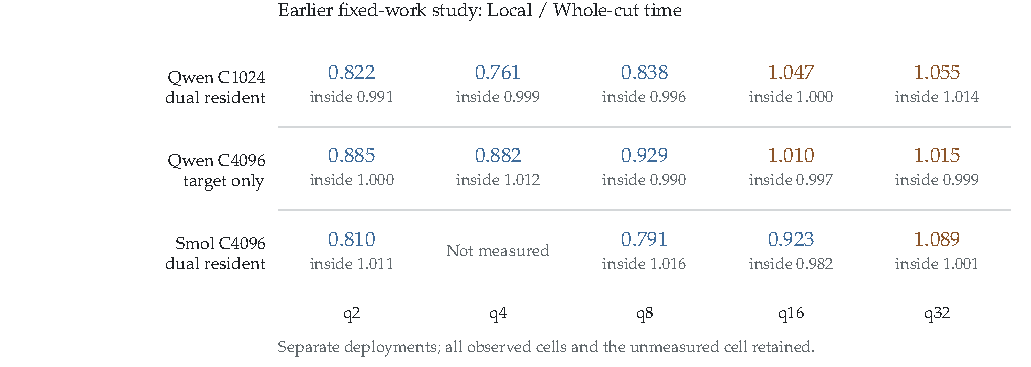
\includegraphics[width=\textwidth]{figures/supp_historical_geometry.pdf}
\caption{Archived Vulkan fixed-work layout geometry. Each labelled cell gives its measured crossing ratio and paired within-bucket control. A grey unmeasured cell is retained as missing, rather than interpolated. This historical configuration differs from the final resident C4096 experiment of Fig.~\ref{fig:vulkan}.}
\label{fig:historical-vulkan}
\end{figure*}

The RTX and B570 natural-prefix panels each use 32 held-out roots and four sessions. Both frozen AUTO policies are constant; neither meets its service-benefit screen, and all three baseline/AUTO intervals include 1. Their file-backed and host-memory snapshot lifecycles remain separate. A subsequent RTX study selects eight unexposed roots with distinguishing whole/rechunk calls before outputs. WB-rechunk/QB is 0.960486 for append and 0.994379 for complete service, with reversed service directions across sessions. These findings motivate the strong whole-rechunk control.

The B570 producer intervention uses eight preselected GSM8K~\cite{gsm8k}/MATH-500 roots, 48 scientific cells and 152 requests. P1-to-P4T changes initial full vectors and serialized state on all eight inputs; consumer compatibility depends on the resulting state, and some pairs still differ from the free reference. In the independent RTX witness, a 704-token prompt yields matching text but different active KV/frontier. A diagnostic $1+3$ split restores the scalar result; it supplies state evidence rather than a new service measurement.



\section{Sources and Reproduction}
The companion repository~\cite{records} supplies implementation snapshots, build recipes, protocols, all fixed controls and statistical records. Table~\ref{tab:source-versions} identifies immutable experimental trees. The author package maps every figure to its source data and regenerates the figures and tables offline.

Its arithmetic reconstruction checks 15 application ratios, all 96 mixed-Q4 request timings, 16 registered q8 interval endpoints from 128 arm/root aggregates, 108 Vulkan append timings, and the added matched-history panel's 128 operations. For the 8B factorial, 64 supplied whole-loop4 request times anchor the other arm/root sums recovered from published paired ratios. These inputs reconstruct four direct intervals and the interaction. The 14B root ratios reconstruct the interaction; its direct intervals and the application intervals are inherited from the source analyses. The strong-loop operator input contains the 36 published paired ratios. Each input's representation and immutable source are recorded in the manifests.

A fresh native numerical replication uses the pinned model and runtime bytes, qualified recipes and independent references. Licensed weights and some large vector/KV captures are held separately, with byte/hash inventories in the public records. Statistical reconstruction reproduces the calculations available in the package. The source protocols preserve failed execution epochs, observer corrections and complete research-cost accounting.
